\chapter{Исследовательский раздел}

\section{Описание исследования}

Целью данного исследования является сравнение времени выполнения запроса на создания нового элемента заказа в зависимости от расположения вычислений: на уровне базы данных или на уровне бизнес логики.

Для добавления нового элемента заказа необходимо проверить, хватает ли вина на складе и не добавлено ли уже такое вино в данный заказ. Для данных проверок был написан триггер, который срабатывает при каждом добавлении элемента заказа. А также реализована еще одна функция вставки на уровне бизнес-логики. С помощью библиотеки Faker\cite{faker} были сгенерированы правдоподобные данные для пользователей. На время исследования количество пользователей постоянно и равно 10. Также были сгенерированы заказы. Их количество тоже постоянно на протяжении всего исследования. В таблице с винами вставлены 3960 вин. Количество элементов заказов в таблице меняется от 10 до 100 с шагом в 10, от 100 до 1000 с шагом 100, от 1000 до 10000 с шагом 1000. Для каждого запуска исследования поднимается свой тестовый контейнер базы данных.

\section{Результат исследования}

Результаты замеров (в мс.) приведены на рисунке \ref{img:resultGraph}. Для получения более достоверных данных, элемент заказа вставлялся 500 раз, а затем бралось среднее значение времени. 

% \includeimage
%     {resultGraph} % Имя файла без расширения (файл должен быть расположен в директории inc/img/)
%     {f} % Обтекание (без обтекания)
%     {h} % Положение рисунка (см. figure из пакета float)
%     {0.8\textwidth} % Ширина рисунка
%     {Сравнение времени проверки нового элемента заказа от расположений вычислений}

\begin{figure}[H]
\vspace{-40pt}
	\centering
	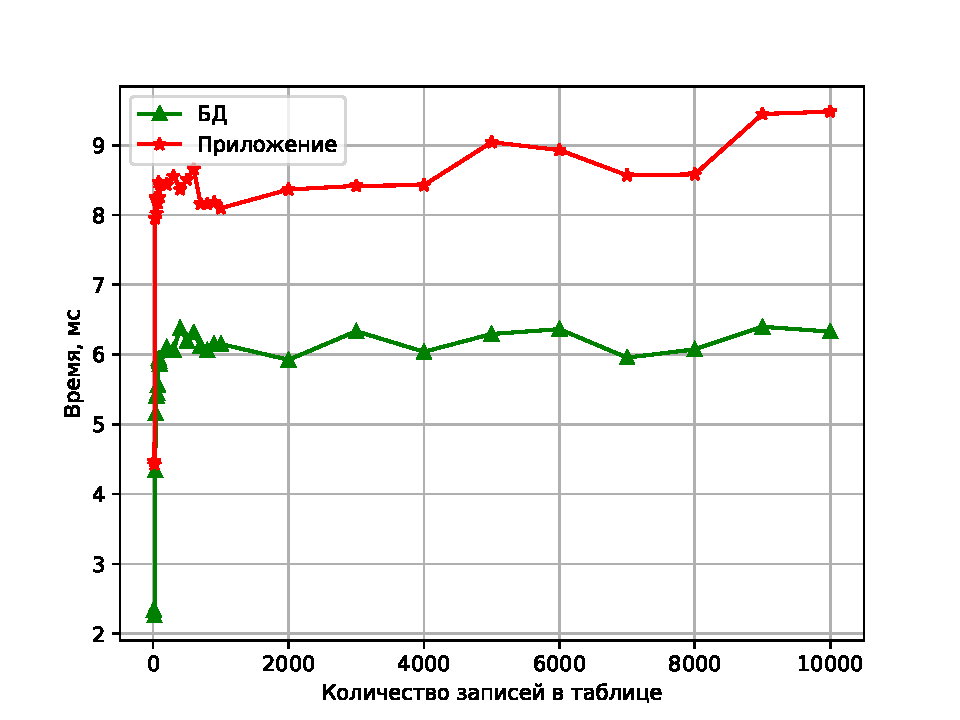
\includegraphics[scale=1]{inc/img/resultGraph.pdf}
	\caption{Сравнение времени проверки нового элемента заказа от расположений вычислений}
	\label{img:res}
\end{figure} 

% \section{Вывод}

% В данном разделе было описано исследование сравнение времени выполнения запроса на создания нового элемента заказа в зависимости от расположения вычислений: на уровне базы данных или на уровне бизнес логики.


По полученным данным можно сказать, что вычисления на уровне базы данных в среднем в полтора раза быстрее, чем на уровне приложения, так как из приложения приходится несколько раз обращаться к базе данных, чтобы получить информацию из разных таблиц.